\documentclass[10pt,a4paper]{article}
\usepackage[utf8]{inputenc}
\usepackage[english]{babel}
\usepackage{amsmath,amsfonts,amssymb}
\usepackage{graphicx}
\usepackage{booktabs}
\usepackage{longtable}
\usepackage{array}
\usepackage{multirow}
\usepackage{multicol}
\usepackage{url}
\usepackage{hyperref}
\usepackage{geometry}
\usepackage{float}
\usepackage{subcaption}
\usepackage{algorithm}
\usepackage{algorithmic}
\usepackage{listings}
\usepackage{xcolor}
\usepackage{setspace}

% Page geometry
\geometry{margin=2.5cm}

% Line spacing 1.5
\onehalfspacing

% Code listing style
\lstset{
    basicstyle=\ttfamily\footnotesize,
    breaklines=true,
    frame=single,
    language=Python,
    showstringspaces=false,
    commentstyle=\color{gray},
    keywordstyle=\color{blue},
    stringstyle=\color{red}
}

\title{Open-Vocabulary Segmentation of Aerial Photos}

\author{Luís Marnoto Lopes}
\date{\today}

\begin{document}

\maketitle

\tableofcontents
\newpage

\section{Introduction}

% [Existing introduction content will be moved here - describes the overall problem, contributions, and scope]



\section{Related Work}

\subsection{Aerial Image Segmentation Datasets}

\subsubsection{Semantic Segmentation Datasets}

% [Content about DeepGlobe, LoveDA, and other semantic segmentation datasets for aerial imagery]

\subsubsection{Instance Segmentation Datasets}

% [Content about iSAID and other instance segmentation datasets for aerial imagery]

\subsubsection{Referring Instance Segmentation Datasets}

% [Content about RefSegRS, RRSIS-D, NWPU-Refer and other referring expression datasets]

\subsection{Model Architectures for Aerial Imagery Segmentation}

\subsubsection{RSRefSeg}

% [Content about RSRefSeg architecture, SigLIP2 + SAM integration, referring expression segmentation capabilities, etc.]

\subsection{Historic Aerial Imagery}

% [Content about historic remote sensing, challenges with historic imagery, processing techniques, etc.]

\subsection{Multimodal Large Language Models}

% [Content about LLM capabilities, generalizability, vision-language models, their application to remote sensing, etc.]



\section{Dataset Construction}

% Dataset sources table
\begin{table}[H]
\centering
\caption{Dataset Source Contributions to AERIAL-D}
\label{tab:dataset_sources}
\begin{tabular}{@{}lrrr@{}}
\toprule
\textbf{Source Dataset} & \textbf{Patches} & \textbf{Individual Instances} & \textbf{Groups} \\
\midrule
iSAID & -- & -- & -- \\
LoveDA & -- & -- & -- \\
DeepGlobe & -- & -- & -- \\
\midrule
\textbf{Total} & \textbf{43,514} & \textbf{128,715} & \textbf{134,202} \\
\bottomrule
\end{tabular}
\end{table}

\subsection{Rule-Based Generation Pipeline}

\begin{figure}[H]
\centering
\begin{minipage}{0.5\textwidth}
\centering
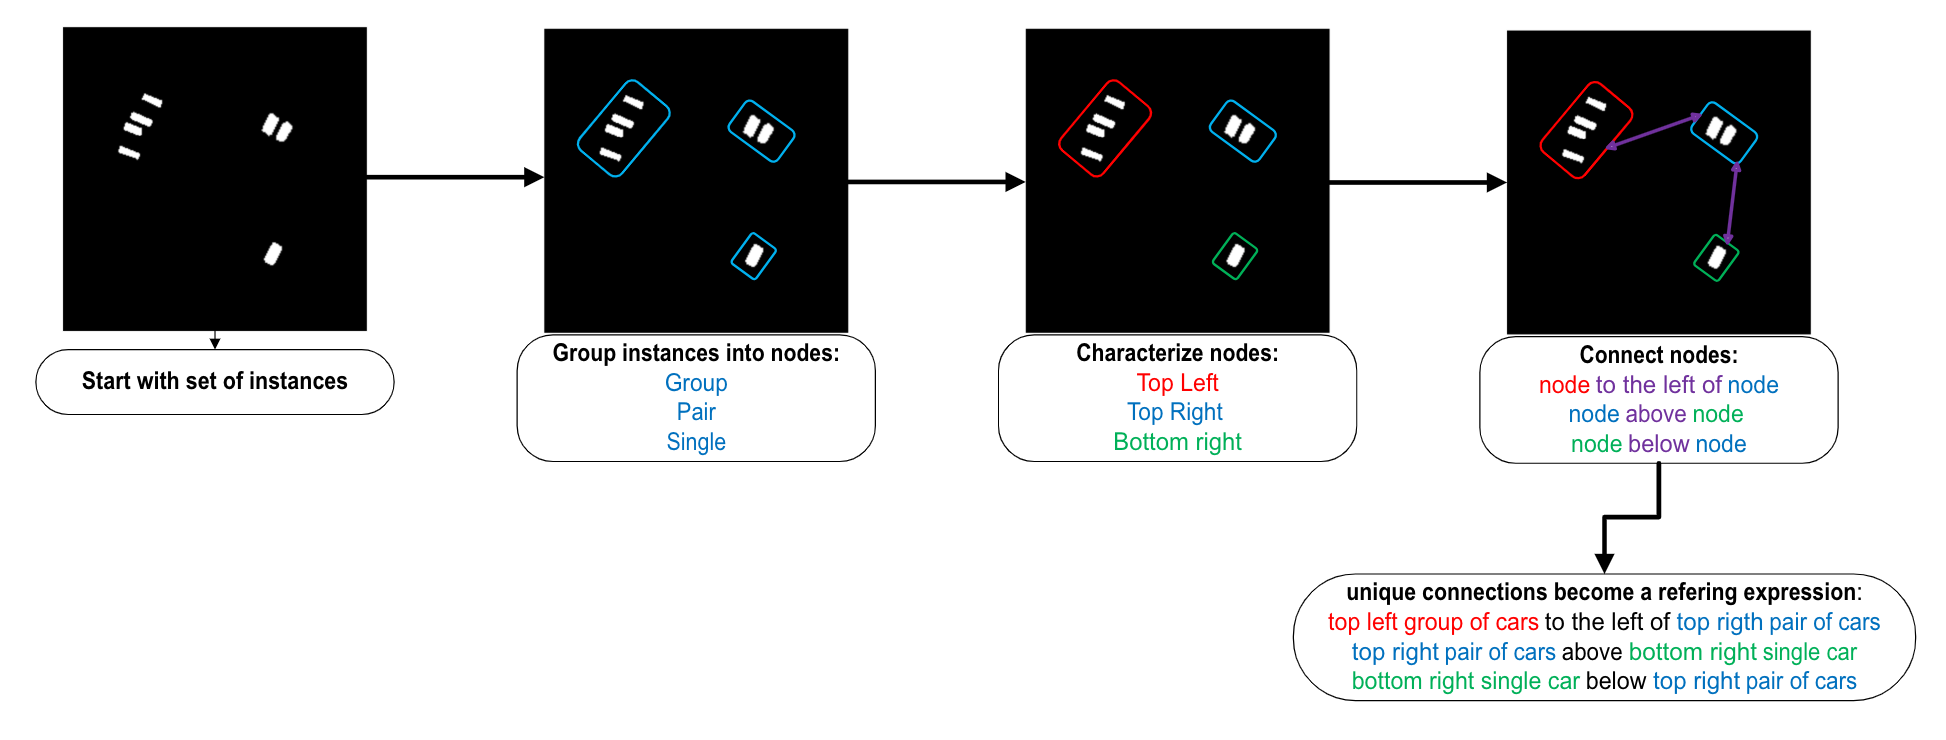
\includegraphics[width=0.7\textwidth]{rule_based_generation.png}
\end{minipage}%
\begin{minipage}{0.5\textwidth}
\centering
\vspace{0.5cm}
\resizebox{\textwidth}{!}{%
\footnotesize
\begin{tabular}{@{}ll@{}}
\toprule
\textbf{Rule Type} & \textbf{Example Instance} \\
\midrule
Category & "plane" \\
Grid Position & "in the top right" \\
Extreme Position & None \\
Size Comparison & None \\
Color Classification & "light" \\
Directional Relations & "to the bottom right of a plane" \\
& "to the top right of a plane" \\
\midrule
\multicolumn{2}{l}{\textbf{Final Expressions}} \\
\multicolumn{2}{l}{"the plane in the top right"} \\
\multicolumn{2}{l}{"the light plane in the top right"} \\
\multicolumn{2}{l}{"the plane in the top right to the bottom right of a plane"} \\
\multicolumn{2}{l}{"the light plane in the top right to the bottom right of a plane"} \\
\multicolumn{2}{l}{"the plane in the top right to the top right of a plane"} \\
\multicolumn{2}{l}{"the light plane in the top right to the top right of a plane"} \\
\bottomrule
\end{tabular}%
}
\end{minipage}
\caption{Example of rule generation for a single instance. The highlighted plane in the top right section demonstrates how the system assigns spatial, visual, and relational rules that will later be combined into referring expressions.}
\label{fig:rule_example}
\end{figure}

Our rule-based component enriches each patch with spatial structure and language-ready annotations before LLM enhancement. It operates on XML annotations produced by the patching steps and outputs three successive datasets: (1) with rules added, (2) with all candidate expressions, and (3) with expressions filtered for uniqueness. Below we summarize the main stages implemented in the pipeline scripts.

\begin{enumerate}
    \item \textbf{Parse instances and metadata}. For every object we read category, bounding box, centroid, area, segmentation (RLE), and a cutoff flag when less than half the object remains inside the patch. This is the starting point for all subsequent rules.
    \item \textbf{Grid positions with borderline handling}. Each patch is partitioned into a 3\,\(\times\,\)3 grid. A center "no-man's land" controlled by \(\alpha = 0.2\) and a small border tolerance mark borderline cases. We assign a primary position label (for example, "in the top left") and, when near cell boundaries, record all alternative positions that might also apply. These alternatives are later expanded into language variants.
    \item \textbf{Extreme positions}. For each category independently we assign topmost, bottommost, leftmost, and rightmost when the leading candidate is separated from the next by at least five percent of the image extent along the corresponding axis. The extreme tag is stored on the instance.
    \item \textbf{Size attributes}. Within each category we detect salient size outliers: an instance is tagged as \emph{largest} if its area exceeds the second largest by a factor of 1.5 or more. The \emph{smallest} tag is assigned only among fully visible instances and under the same 1.5\,\(\times\) separation rule.
    \item \textbf{Local relationships between instances}. We compute pairwise spatial relations only to nearby targets using a dynamic radius equal to a base value plus a size-dependent term. Relations cover eight directions (left/right, above/below, and diagonals). A 15-degree angular overlap yields borderline relations that store multiple admissible directions; otherwise a single direction is stored. Containment cases (one box or centroid inside the other) are ignored. We keep distance for optional text rendering and mark if either endpoint is cutoff.
    \item \textbf{Clustering into groups}. Instances are clustered \emph{per category} using DBSCAN with a distance based on minimum bbox separation, producing multi-instance groups while capping oversized clusters. We create single-instance groups only when they participate in relations with multi-instance groups. For each group we compute centroid, grid position, size, and a combined segmentation mask.
    \item \textbf{Higher-level groups}. We add class-level groups that aggregate all instances of the same class present in the patch (semantic "all X in the image" expressions). We also form a special pair group that merges small and large vehicles when both are present.
    \item \textbf{Group relationships}. We compute relations among groups and between groups and single-instance groups (but not single-to-single), using the same directional scheme and distance gating as for instances while avoiding containment.
    \item \textbf{Color reasoning with ambiguity}. For each instance we sample HSV pixels from its segmentation and determine a dominant color. Achromatic detection uses a saturation threshold; brightness separates light from dark. Chromatic categories are assigned only when a single hue dominates; otherwise the color is marked ambiguous and we retain a small set of candidate terms. To avoid artifacts, chromatic colors are suppressed for buildings and water; only light/dark are kept for those classes.
    \item \textbf{Expression generation}. From the attributes above we synthesize comprehensive referring expressions for \emph{instances} and \emph{groups}. We enumerate combinations of category, grid position, relationships, extremes, size, and color. Borderline positions and borderline relationships expand into multiple variants. Expressions associated with cutoff objects or ambiguous color are tracked as "dummy" for potential removal.
    \item \textbf{Uniqueness filtering and cleanup}. We standardize class names (and plurals), collapse "group of 1" into the singular, and remove any expression text that appears more than once across the patch—if a phrase is duplicated, \emph{all} of its occurrences are dropped. We then discard color expressions for ambiguous objects, delete any object or group with no expressions left, and remove corresponding images when a patch becomes empty. Finally we strip intermediate rule fields from XML, leaving clean annotations with only unique expressions.
\end{enumerate}

% Expression taxonomy table
\begin{table}[H]
\centering
\caption{Complete Taxonomy of Generated Expression Types}
\label{tab:expression_types}
\resizebox{\textwidth}{!}{%
\begin{tabular}{@{}lll@{}}
\toprule
\textbf{Expression Type} & \textbf{Description} & \textbf{Example} \\
\midrule
\multicolumn{3}{l}{\textbf{Individual Instance Expressions}} \\
\midrule
Category Only & Basic object category & "the ship" \\
Category + Position & Category with grid position & "the ship in the bottom right" \\
Category + Position + Relationship & Category with position and spatial relationship & "the ship in the bottom right that is to the left of a harbor" \\
Extreme Position + Category & Extreme spatial position with category & "the topmost ship" \\
Extreme + Category + Position & Extreme position with grid location & "the topmost ship in the top left" \\
Extreme + Category + Position + Relationship & Extreme position with relationship & "the topmost ship in the top left that is above a building" \\
Size + Category + Position & Size attribute with position & "the largest ship in the bottom right" \\
Size + Category + Position + Relationship & Size attribute with relationship & "the largest ship in the bottom right that is above a harbor" \\
Size + Extreme + Category + Position & Size with extreme position & "the largest topmost ship in the top left" \\
Size + Extreme + Category + Position + Relationship & All attributes combined & "the largest topmost ship in the top left that is above a building" \\
Color + Category & Color attribute with category & "the dark ship" \\
Color + Category + Position & Color with position & "the dark ship in the bottom right" \\
Color + Category + Position + Relationship & Color with relationship & "the dark ship in the bottom right that is to the left of a harbor" \\
Color + Extreme + Category & Color with extreme position & "the dark topmost ship" \\
Color + Extreme + Category + Position & Color with extreme and position & "the dark topmost ship in the top left" \\
Color + Extreme + Category + Position + Relationship & Color with all spatial attributes & "the dark topmost ship in the top left that is above a building" \\
Color + Size + Category + Position & Color with size attribute & "the dark largest ship in the bottom right" \\
Color + Size + Category + Position + Relationship & Color with size and relationship & "the dark largest ship in the bottom right that is above a harbor" \\
Color + Size + Extreme + Category + Position & All attributes with color & "the dark largest topmost ship in the top left" \\
Color + Size + Extreme + Category + Position + Relationship & Maximum complexity expression & "the dark largest topmost ship in the top left that is above a building" \\
\midrule
\multicolumn{3}{l}{\textbf{Group Expressions}} \\
\midrule
Basic Group & Group with size and category & "the group of 3 ships in the center" \\
Group + Extreme Position & Group with extreme spatial position & "the topmost group of 3 ships in the center" \\
Group + Relationship & Group with spatial relationship to other groups & "the group of 3 ships in the center that is above a group of 2 buildings" \\
Single Instance + Group Relationship & Individual object referencing group & "the ship in the bottom right that is to the left of a group of 2 harbors" \\
Class-Level Groups & Semantic segmentation expressions & "all buildings in the image" \\
Special Combination Groups & Multi-class semantic groups & "all small and large vehicles in the image" \\
\bottomrule
\end{tabular}%
}
\end{table}

\subsection{LLM Enhancement Component}

% LLM enhancement example figure
\begin{figure}[H]
\centering
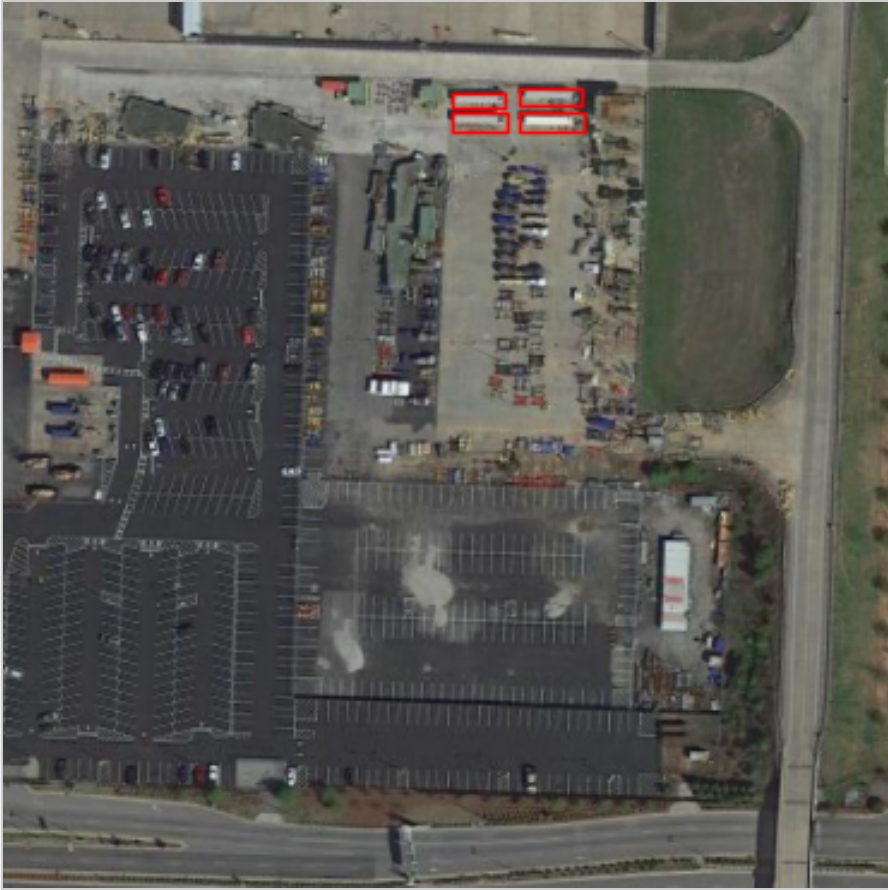
\includegraphics[width=0.4\textwidth]{example_group.png}
\caption{Example aerial image showing a group of four large vehicles (highlighted in red boxes) that demonstrates the LLM enhancement process.}
\label{fig:llm_enhancement_example}
\end{figure}

% LLM enhancement example table
\begin{table}[H]
\centering
\caption{Example LLM Enhancement Output for Group Instance}
\label{tab:llm_enhancement_example}
\begin{tabular}{@{}p{0.25\textwidth}p{0.7\textwidth}@{}}
\toprule
\textbf{Enhancement Type} & \textbf{Expression} \\
\midrule
Original Expression & the group of 4 large vehicles in the top center \\
\midrule
Enhanced Expression & the cluster of four big vehicles near the upper middle \\
\midrule
\multirow{2}{0.25\textwidth}{Unique Expressions} & the four large vehicles lined up side by side just below the pale paved strip at the very top middle \\
\cmidrule(l){2-2}
& the set of four big vehicles parked in a single row in the upper center beside the grassy area to the right \\
\bottomrule
\end{tabular}
\end{table}



\section{Evaluation Setup}

\subsection{Model Architecture Implementation}

% RSRefSeg architecture figure
\begin{figure}[H]
\centering
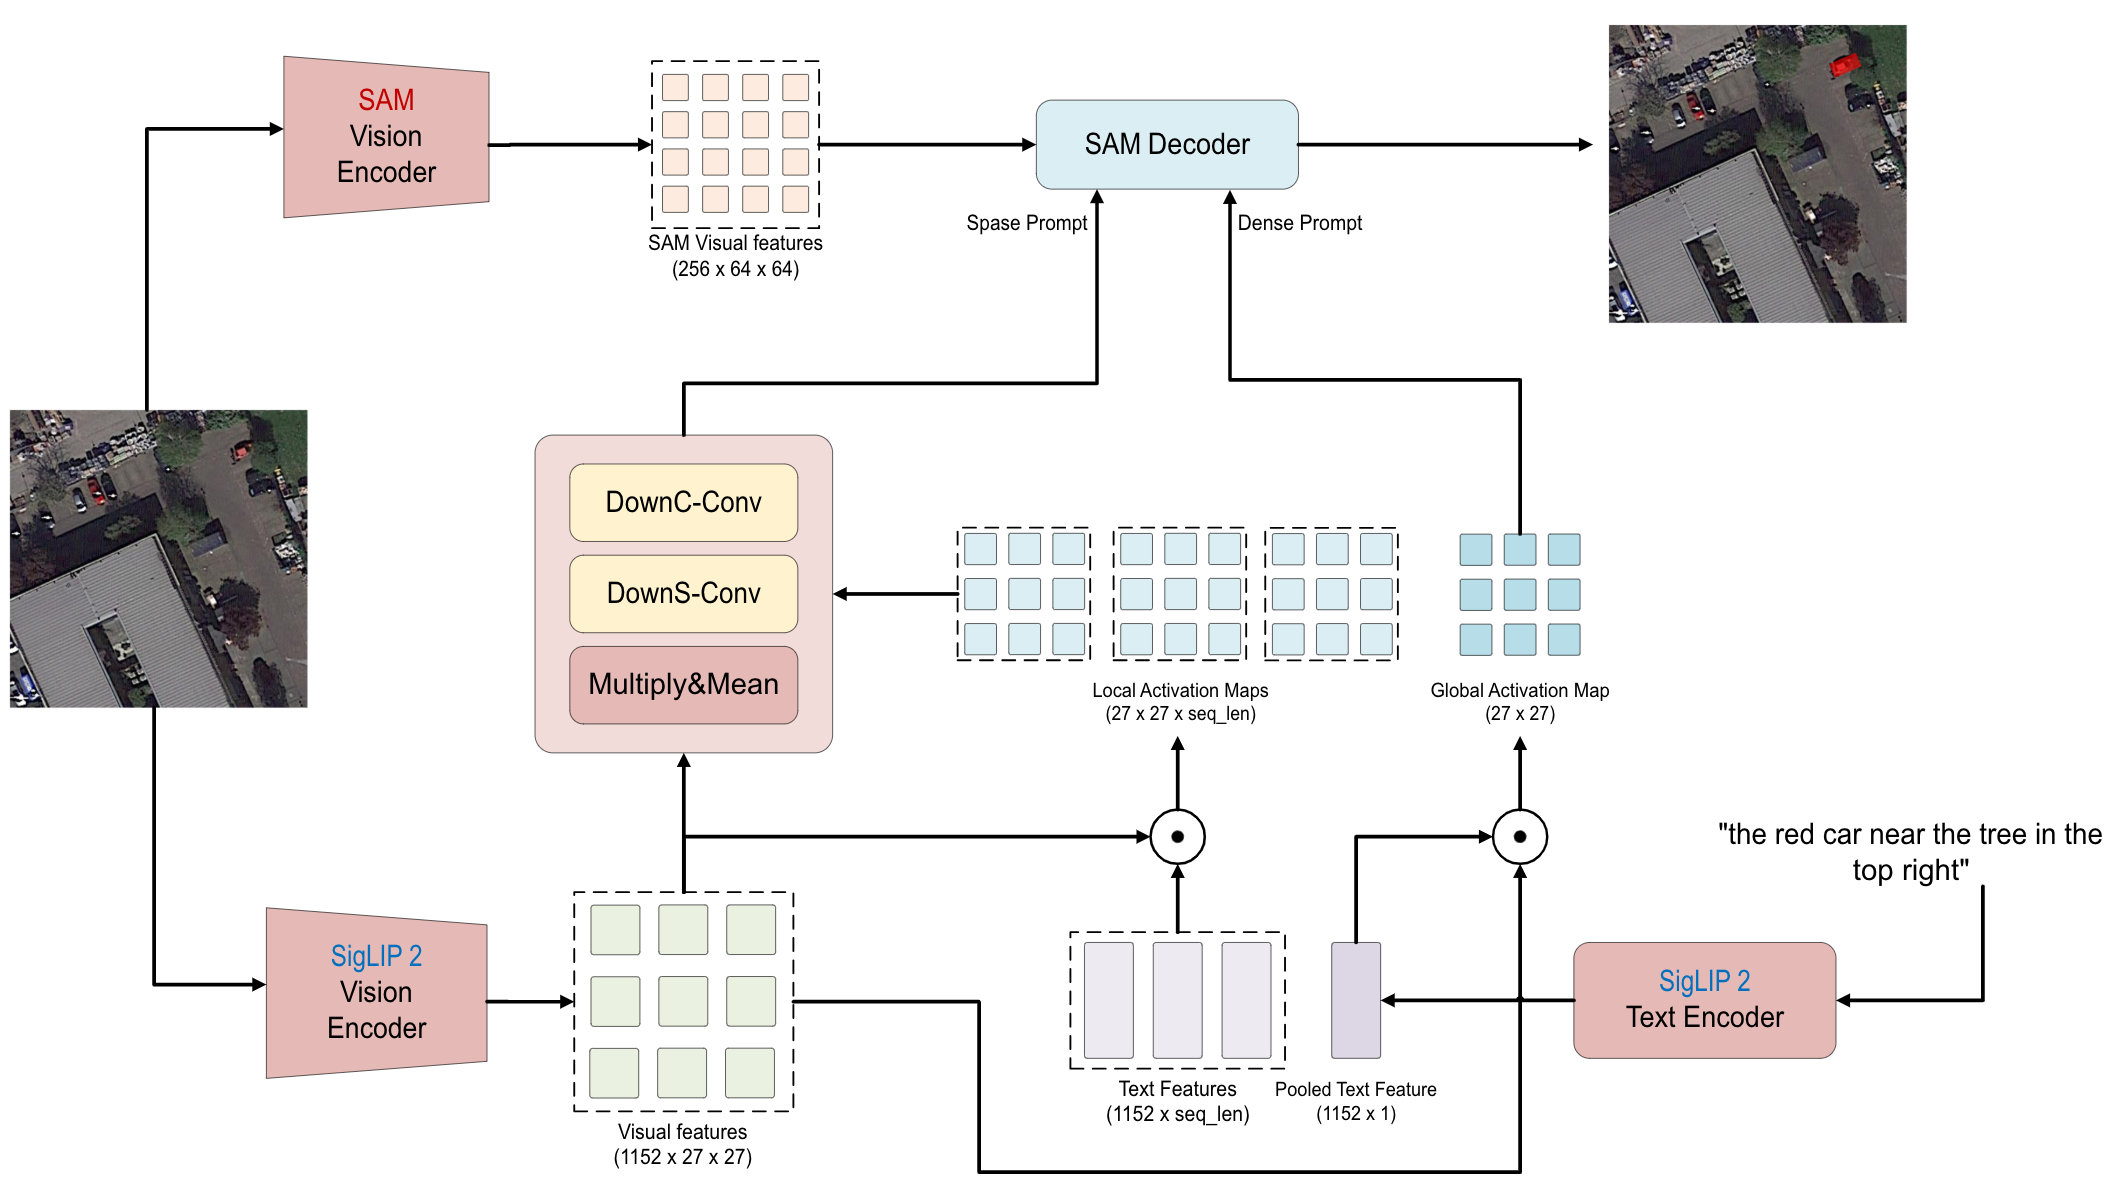
\includegraphics[width=\textwidth]{clipsam.png}
\caption{ClipSAM architecture overview showing the integration of SigLIP2 vision-language encoder with SAM mask decoder through custom prompter networks for text-guided segmentation. The dual-pathway design processes both local (token-level) and global (sentence-level) text-visual interactions to generate sparse and dense prompts for precise aerial image segmentation.}
\label{fig:rsrefseg_architecture}
\end{figure}

\subsection{Dataset Statistics}

% Dataset examples figure
\begin{figure}[H]
\centering
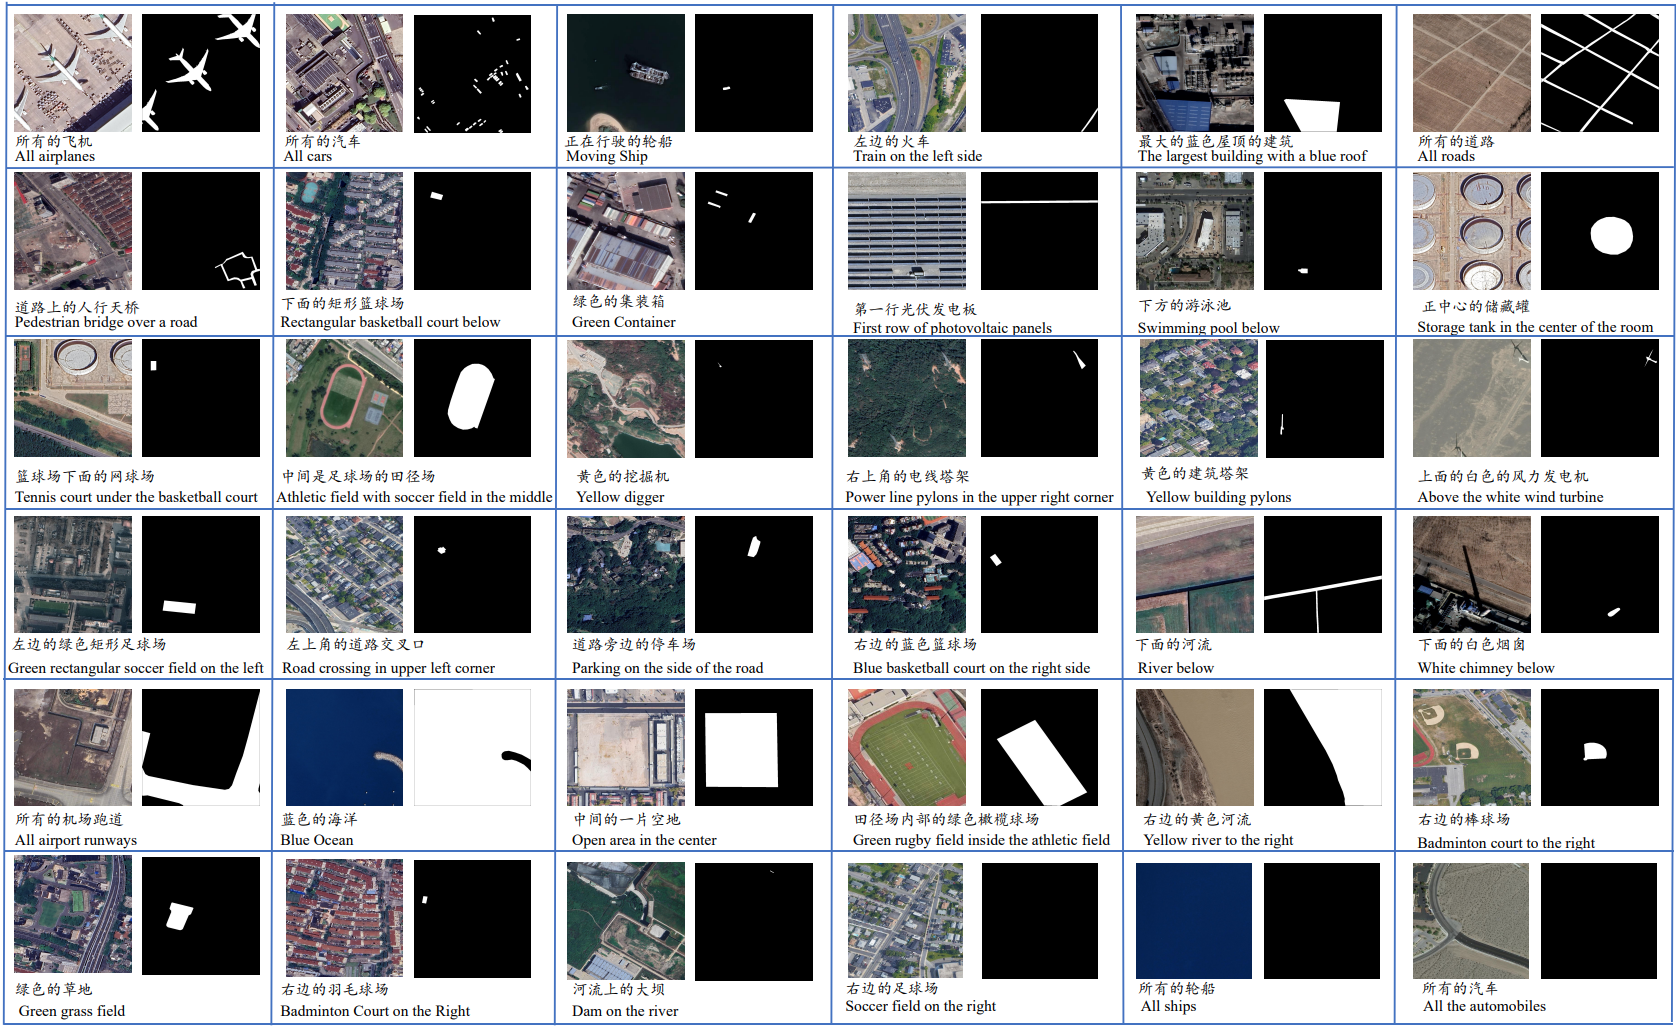
\includegraphics[width=\textwidth]{dataset.png}
\caption{Representative examples from AERIAL-D dataset showing diverse referring expressions with corresponding aerial images and ground truth masks.}
\label{fig:dataset_examples}
\end{figure}

% Dataset statistics table
\begin{table}[H]
\centering
\caption{Dataset Statistics Summary}
\label{tab:dataset_stats}
\begin{tabular}{@{}lrrr@{}}
\toprule
\textbf{Metric} & \textbf{Train} & \textbf{Val} & \textbf{Total} \\
\midrule
Total Patches & 32,460 & 11,054 & 43,514 \\
Individual Objects with Expressions & 94,179 & 34,536 & 128,715 \\
Individual Expressions & 651,098 & 244,210 & 895,308 \\
Groups with Expressions & 99,986 & 34,216 & 134,202 \\
Group Expressions & 487,214 & 163,472 & 650,686 \\
Total Samples & 1,138,312 & 407,682 & 1,545,994 \\
Avg. Expressions per Individual Object & 6.91 & 7.07 & 6.96 \\
Avg. Expressions per Group & 4.87 & 4.78 & 4.85 \\
\bottomrule
\end{tabular}
\end{table}

\subsection{Category Distribution}

% Category distribution table
\begin{table}[H]
\centering
\caption{Object Category Distribution by Instance Type and Source Dataset}
\label{tab:category_dist}
\resizebox{\textwidth}{!}{%
\begin{tabular}{@{}lrrrrr@{}}
\toprule
\textbf{Category} & \textbf{Individual Instances} & \textbf{Groups} & \textbf{Instance Expressions} & \textbf{Group Expressions} & \textbf{Source Dataset} \\
\midrule
Ship & -- & -- & -- & -- & iSAID \\
Large Vehicle & -- & -- & -- & -- & iSAID \\
Small Vehicle & -- & -- & -- & -- & iSAID \\
Building & -- & -- & -- & -- & iSAID \\
Storage Tank & -- & -- & -- & -- & iSAID \\
Harbor & -- & -- & -- & -- & iSAID \\
Swimming Pool & -- & -- & -- & -- & iSAID \\
Tennis Court & -- & -- & -- & -- & iSAID \\
Soccer Ball Field & -- & -- & -- & -- & iSAID \\
Roundabout & -- & -- & -- & -- & iSAID \\
Basketball Court & -- & -- & -- & -- & iSAID \\
Bridge & -- & -- & -- & -- & iSAID \\
Ground Track Field & -- & -- & -- & -- & iSAID \\
Plane & -- & -- & -- & -- & iSAID \\
Helicopter & -- & -- & -- & -- & iSAID \\
Building & -- & -- & -- & -- & LoveDA \\
Water & -- & -- & -- & -- & LoveDA \\
Barren Land & -- & -- & -- & -- & LoveDA \\
Agricultural Area & -- & -- & -- & -- & LoveDA \\
Forest Area & -- & -- & -- & -- & LoveDA \\
Road & -- & -- & -- & -- & DeepGlobe \\
\bottomrule
\end{tabular}%
}
\end{table}

\subsection{Expression Type Analysis}

Table~\ref{tab:expression_type_dist} shows the distribution of different expression types generated across the pipeline, including rule-based expressions and LLM enhancements.

% Expression type distribution table
\begin{table}[H]
\centering
\caption{Expression Type Distribution}
\label{tab:expression_type_dist}
\resizebox{\textwidth}{!}{%
\begin{tabular}{@{}ccccccr@{}}
\toprule
\textbf{Category} & \textbf{Position} & \textbf{Extreme} & \textbf{Size} & \textbf{Color} & \textbf{Relationship} & \textbf{Total Count} \\
\midrule
\multicolumn{7}{l}{\textbf{Rule-Based Individual Instance Expressions}} \\
\midrule
\checkmark & & & & & & -- \\
\checkmark & \checkmark & & & & & -- \\
\checkmark & \checkmark & & & & \checkmark & -- \\
\checkmark & & \checkmark & & & & -- \\
\checkmark & \checkmark & \checkmark & & & & -- \\
\checkmark & \checkmark & \checkmark & & & \checkmark & -- \\
\checkmark & \checkmark & & \checkmark & & & -- \\
\checkmark & \checkmark & & \checkmark & & \checkmark & -- \\
\checkmark & \checkmark & \checkmark & \checkmark & & & -- \\
\checkmark & \checkmark & \checkmark & \checkmark & & \checkmark & -- \\
\checkmark & & & & \checkmark & & -- \\
\checkmark & \checkmark & & & \checkmark & & -- \\
\checkmark & \checkmark & & & \checkmark & \checkmark & -- \\
\checkmark & & \checkmark & & \checkmark & & -- \\
\checkmark & \checkmark & \checkmark & & \checkmark & & -- \\
\checkmark & \checkmark & \checkmark & & \checkmark & \checkmark & -- \\
\checkmark & \checkmark & & \checkmark & \checkmark & & -- \\
\checkmark & \checkmark & & \checkmark & \checkmark & \checkmark & -- \\
\checkmark & \checkmark & \checkmark & \checkmark & \checkmark & & -- \\
\checkmark & \checkmark & \checkmark & \checkmark & \checkmark & \checkmark & -- \\
\midrule
\multicolumn{7}{l}{\textbf{Rule-Based Group Expressions}} \\
\midrule
\checkmark & \checkmark & & & & & -- \\
\checkmark & \checkmark & \checkmark & & & & -- \\
\checkmark & \checkmark & & & & \checkmark & -- \\
\checkmark & \checkmark & & & & \checkmark & -- \\
\checkmark & & & & & & -- \\
\checkmark & & & \checkmark & & & -- \\
\bottomrule
\end{tabular}%
}
\end{table}

\subsection{LLM Enhancement Statistics}

% LLM enhancement stats table
\begin{table}[H]
\centering
\caption{LLM Enhancement Expression Distribution}
\label{tab:llm_enhancement_stats}
\begin{tabular}{@{}lrrr@{}}
\toprule
\textbf{Expression Source} & \textbf{Train} & \textbf{Val} & \textbf{Total} \\
\midrule
Rule-Based Expressions & -- & -- & -- \\
LLM Enhanced (Language Variations) & -- & -- & -- \\
LLM Unique (Visual Details) & -- & -- & -- \\
\midrule
\textbf{Total Expressions} & \textbf{--} & \textbf{--} & \textbf{--} \\
\bottomrule
\end{tabular}
\end{table}

\subsection{Training Configuration}

% [Training parameters, optimization settings, data splits, augmentation strategies, etc.]

\subsection{Evaluation Methodology}

% [Metrics, validation splits, cross-dataset testing, ablation study design, etc.]



\section{Results}

\subsection{Quantitative Evaluation}

% Cross-dataset performance table
\begin{table}[H]
\centering
\caption{Cross-Dataset Performance Evaluation on Validation Sets}
\label{tab:cross_dataset_results}
\begin{tabular}{@{}lccccc@{}}
\toprule
\textbf{Dataset} & \textbf{IoU@0.5} & \textbf{IoU@0.7} & \textbf{IoU@0.9} & \textbf{mIoU} & \textbf{oIoU} \\
\midrule
AERIAL-D & -- & -- & -- & -- & -- \\
RefSegRS & -- & -- & -- & -- & -- \\
RRSIS-D & -- & -- & -- & -- & -- \\
NWPU-Refer & -- & -- & -- & -- & -- \\
\bottomrule
\end{tabular}
\end{table}

% Dataset comparison table
\begin{table}[H]
\centering
\caption{Comparison with Existing RRSIS Datasets}
\label{tab:dataset_comparison}
\resizebox{\textwidth}{!}{%
\begin{tabular}{@{}lccccccr@{}}
\toprule
\textbf{Dataset} & \textbf{Image Resolution} & \textbf{Images} & \textbf{Annotations} & \textbf{Single-object} & \textbf{Multi-object} & \textbf{Resolution} & \textbf{Annotation Generation} \\
\midrule
RefSegRS & 0.13m & 4420 & 4420 & \checkmark & $\times$ & 512 & Manual \\
RRSIS-D & 0.5m-30m & 17402 & 17402 & \checkmark & $\times$ & 800 & Semi-auto \\
NWPU-Refer & 0.12m-0.5m & 15003 & 49745 & \checkmark & \checkmark & 1024-2048 & Manual \\
\midrule
\textbf{AERIAL-D} & \textbf{0.3m-2m} & \textbf{43,514} & \textbf{1,545,994} & \textbf{\checkmark} & \textbf{\checkmark} & \textbf{480} & \textbf{Automated + LLM} \\
\bottomrule
\end{tabular}%
}
\end{table}

\subsection{Qualitative Analysis}

% Qualitative examples figure
\begin{figure}[H]
\centering
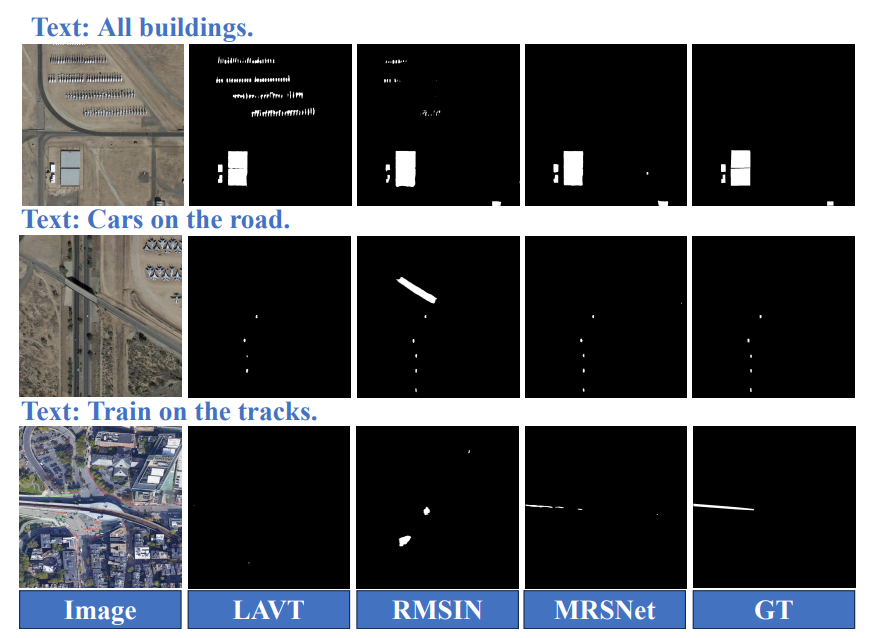
\includegraphics[width=\textwidth]{qualitative.png}
\caption{Qualitative segmentation results from RSRefSeg model on AERIAL-D validation set.}
\label{fig:qualitative_examples}
\end{figure}

% Dataset errors figure
\begin{figure}[H]
\centering
\includegraphics[width=\textwidth]{errors.png}
\caption{Dataset error analysis examples for LLM-generated unique expressions.}
\label{fig:dataset_errors}
\end{figure}

\subsection{Ablation Studies}

% Ablation expression types table
\begin{table}[H]
\centering
\caption{Ablation Study: Expression Type Training Analysis}
\label{tab:ablation_expression_types}
\resizebox{\textwidth}{!}{%
\begin{tabular}{@{}lcccccc@{}}
\toprule
\textbf{Training Configuration} & \textbf{IoU@0.5} & \textbf{IoU@0.7} & \textbf{IoU@0.9} & \textbf{mIoU} & \textbf{oIoU} & \textbf{Training Expressions} \\
\midrule
Rule-based Only & -- & -- & -- & -- & -- & -- \\
Language Variations & -- & -- & -- & -- & -- & -- \\
Unique Expressions & -- & -- & -- & -- & -- & -- \\
Combined All & -- & -- & -- & -- & -- & -- \\
\bottomrule
\end{tabular}%
}
\end{table}



\section{Conclusion}

% [Summary of contributions, impact, limitations, future work, etc.]



\section*{Acknowledgments}

% [Acknowledgments content]




\bibliographystyle{plain}
\bibliography{references}

\appendix

\section{Pipeline Implementation Details}

% [Detailed algorithms, specifications, etc.]

\section{LLM Enhancement Prompts}

% [Complete prompt specifications, examples, etc.]




\end{document} 